\begin{figure}[H]
\centering
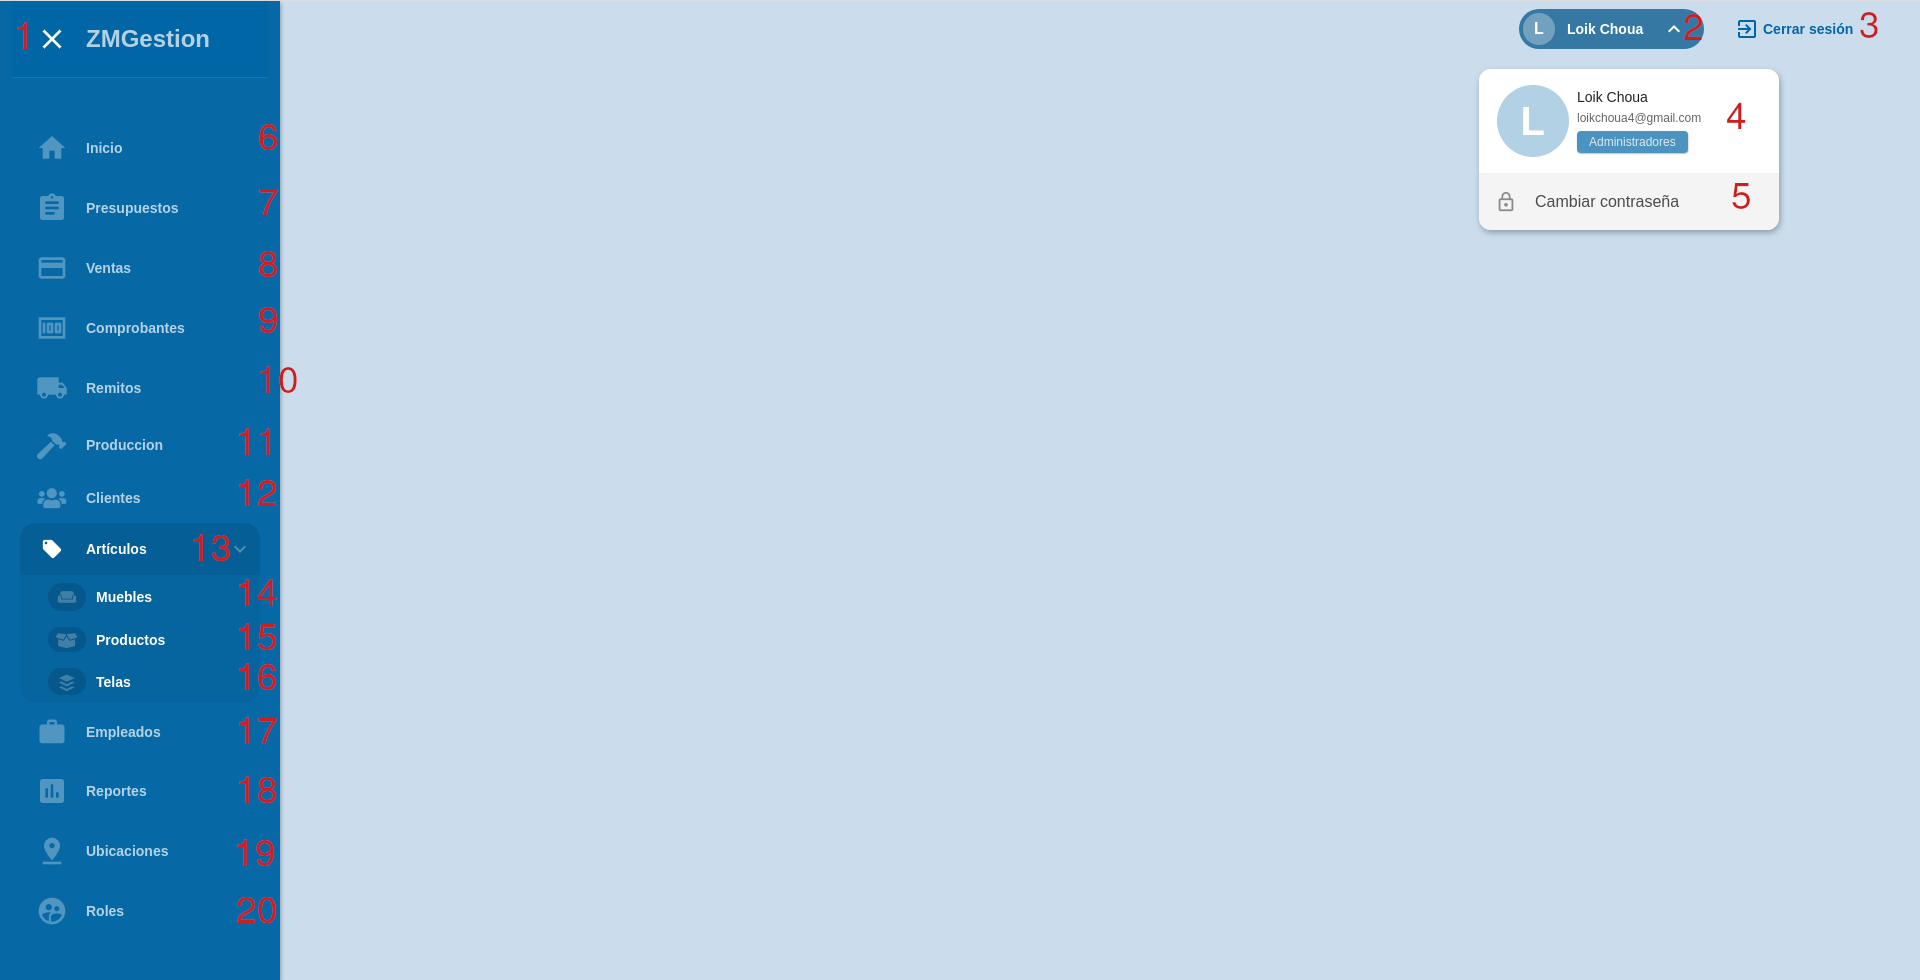
\includegraphics[width=\textwidth,height=\textheight,keepaspectratio]{Escenarios/AD-02-00}
\caption{Escenario - AD-02-00}
\label{fig:AD-02-00}
\end{figure}
Este es el escenario principal de ZMGestion. El botón \textbf{AD-02-01} permite abrir y cerrar el menú lateral, en caso de encontrarse abierto el botón \textbf{AD-02-01} tiene el icono \faTimes y cuando esta cerrado tiene el icono \faBars.
El botón \textbf{AD-02-02} permite abrir y cerrar un menú desplegable en donde el campo \textbf{AD-02-04} muestra información del usuario (nombre, apellido, correo electónico y rol) que inicio sesón en ZMGestion. El botón \textbf{AD-02-05} permite navegar al escenario \textbf{AD-51-00}. 
El botón \textbf{AD-02-03} permite al usuario cerrar sesión en ZMGestion.
En el menú lateral tene,os todos los botones que permiten navegar a diferentes escenarios.
\begin{itemize}
    \item \textbf{AD-02-07}: permite navegar al escenario \textbf{AD-03-00}.
    \item \textbf{AD-02-08}: permite navegar al escenario \textbf{AD-10-00}.
    \item \textbf{AD-02-09}: permite navegar al escenario \textbf{AD-14-00}.
    \item \textbf{AD-02-10}: permite navegar al escenario \textbf{AD-16-00}.
    \item \textbf{AD-02-11}: permite navegar al escenario \textbf{AD-22-00}.
    \item \textbf{AD-02-12}: permite navegar al escenario \textbf{AD-28-00}.
    \item \textbf{AD-02-07}: despliega un menú que permite visualizar los botones:
    \begin{itemize}
        \item \textbf{AD-02-14}: permite navegar al escenario \textbf{AD-48-00}.
        \item \textbf{AD-02-15}: permite navegar al escenario \textbf{AD-42-00}. 
        \item \textbf{AD-02-16}: permite navegar al escenario \textbf{AD-39-00}.
    \end{itemize}
    \item \textbf{AD-02-17}: permite navegar al escenario \textbf{AD-32-00}.
    \item \textbf{AD-02-19}: permite navegar al escenario \textbf{AD-37-00}.
    \item \textbf{AD-02-20}: permite navegar al escenario \textbf{AD-35-00}.
\end{itemize}
\clearpage
